\documentclass[12pt,letterpaper]{article}
\usepackage{fullpage}
\usepackage[top=2cm, bottom=4cm, left=2.5cm, right=2.5cm]{geometry}
\usepackage{amsmath,amsthm,amsfonts,amssymb,amscd}
\usepackage{lastpage}
\usepackage{enumerate}
\usepackage{fancyhdr}
\usepackage{mathrsfs}
\usepackage{xcolor}
\usepackage{graphicx}
\usepackage{listings}
\usepackage{hyperref}
\usepackage{float}

\hypersetup{%
  colorlinks=true,
  linkcolor=blue,
  linkbordercolor={0 0 1}
}
 
\renewcommand\lstlistingname{Algorithm}
\renewcommand\lstlistlistingname{Algorithms}
\def\lstlistingautorefname{Alg.}

\lstdefinestyle{Python}{
    language        = Python,
    frame           = lines, 
    basicstyle      = \footnotesize,
    keywordstyle    = \color{blue},
    stringstyle     = \color{green},
    commentstyle    = \color{red}\ttfamily
}

\setlength{\parindent}{0.0in}
\setlength{\parskip}{0.05in}
\begin{document}
    Homework 1\\
    Name: Sunny Lee

    \begin{enumerate}
        \item \emph{Solution.}
            \begin{enumerate}
                \item $T_{2}(x) = x^2 + x$
                \item Using the Taylor polynomial above, we see that the integral from 0 to .5
                of our Taylor Polynomial is: 

                \begin{eqnarray*}
                    \int_{0}^{.5} x + x^2 = \frac{x^2}{2} + \frac{x^3}{3} \Big|_0^{.5} = \frac{1}{6}
                \end{eqnarray*}
                To find our error bound, we must first find where our error term is largest on the interval $[0, .5]$.
                By plotting the error bound function: 
                \begin{eqnarray}
                    f^{(3)}(x) = \frac{6x}{(x-1)^4} - \frac{6}{(x-1)^3}
                \end{eqnarray}
                we see that the highest amount of error on our interval $[0, .5]$is going to be at $.5$
                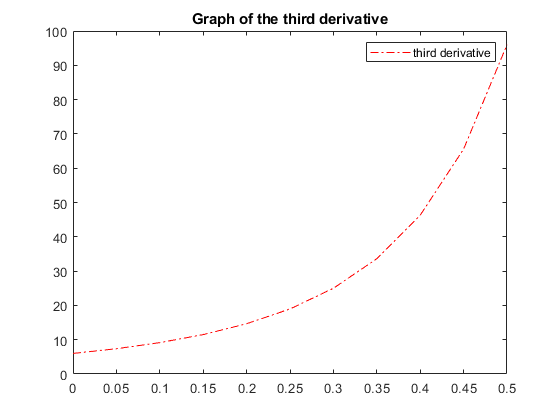
\includegraphics{third derivative.png}

                Therefore, we can use $x = .5$ in our error term to get: 
                \begin{eqnarray*}
                    f^{(3)}(.5) = \frac{6(.5)}{((.5)-1)^4} - \frac{6}{((.5)-1)^3} = 96
                \end{eqnarray*}
                
                Finally, we can use this value and take the integral of our error term to get an error bound:
                \begin{eqnarray*}
                    errorbound = \int_{0}^{.5} \frac{96x^3}{3!}dx = \frac{1}{4}
                \end{eqnarray*}

                Which gives us an actual error of: 
                \begin{eqnarray*}
                    error = \int_{0}^{.5} \frac{x}{1-x} - \int_{0}^{.5} x + x^2 = \frac{2\ln(2)-1}{2} - \frac{1}{6} \approx 0.02648 < \frac{1}{4}
                \end{eqnarray*}

                and we see this error is much less than our error bound found above. 
            \end{enumerate}
        \item \emph{Solution.} \\
            $f(x)$ is a polynomial, therefore it is continuous on the interval $(-\inf, \inf)$.
            Taking the derivative of $f$, we see the derivative can never reach zero: 
            \begin{eqnarray*}
                f(x) = 4x^5 + x^3 + 7x -2\\
                f'(x) = 20x^4 + 3x^2 + 7 \geq 7 > 0
            \end{eqnarray*}
            For every x. Since this function is a monotonically increasing function, 
            we can make use of Rolle's Theorem to show this function cannot have more
            than two solutions. We can also show that this function has at least one 
            solution by taking the function at $0$ and $1$: 

            \begin{eqnarray*}
                f(0) = -2\\
                f(1) = 10
            \end{eqnarray*}

            By the intermediate value theorem, we see this function has a root somewhere 
            between (0, 1)
        \item \emph{Solution.} \\
            By taking the function at the endpoints of our interval, 
            \begin{eqnarray*}
                f(0) = -1\\
                f(2) = 11
            \end{eqnarray*}
            We see the function changes sign at the two endpoints. Using the Intermediate
            Value Theorem, and the fact that polynomials are continuous, we know the function
            will hit every point between $[-1, 11]$. Therefore, the function at somepoint
            in the interval $[0, 2]$ will be zero. 
        
        \item \emph{Solution.} 
            \begin{enumerate}
                \item 
                Suppose f $\in$ C[a, b] and that $x_{1}$ and $x_{2}$ are in $[a, b]$. Then,
                because $f$ is continuous, we know that $f$ hits every value between $[f(a), f(b)]$
                and because $x_{1}$ and $x_{2}$ are within $a$ and $b$, we know that every point 
                in $[f(x_{1}), f(x_{2})]$ is also hit. We also know $\frac{f(x_{1}) + f(x_{2})}{2}$
                is an average of $f(x_{1})$ and $f(x_{2})$, therefore $f(\xi) \in [f(x_{1}), f(x_{2})]$.
                Since $f(\xi)$ is between the two values $f(x_{1}), f(x_{2})$, we know, by the IVT,
                that there must exist a $\xi$ somewhere between $x_{1}$ and $x_{2}$.
                
                \item
                Similar to what was mentioned above, we know $f(\xi)$ must be between 
                $[c_{1}f(x_{1}), c_{2}f(x_{2})]$, as again, the value $c_{1}f(x_{1}) + c_{2}f(x_{2})$
                is divided by the two constants $c_{1} + c_{2}$, which is a weighted average. Therefore, $f(\xi)$ exists between the two 
                values $[c_{1}f(x_{1}), c_{2}f(x_{2})]$. Thus, by the IVT, we know $\xi$ 
                must exist somewhere between $x_{1}$ and $x_{2}$.
            \end{enumerate}
            
            
    \end{enumerate}

\end{document}
